\begin{enumerate}[label=\thechapter.\arabic*,ref=\thechapter.\theenumi]
\item
For the circuit given below, choose the angular frequency $ \omega_0$ at which voltage across capacitor has maximum amplitude?
\begin{figure}[h!]
    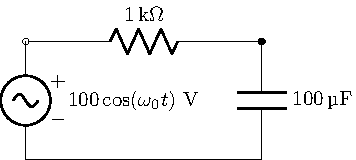
\includegraphics[width = 0.5\columnwidth]{2023/BM/16/figs/c_fig1.pdf}
    \caption{circuit }
    \centering
    \label{fig: bm_16_fig_1}
\end{figure}
\begin{enumerate}
    \item[(A)] 1000
    \item[(B)] 100
    \item[(C)] 1
    \item[(D)] 0   
\end{enumerate}
\hfill(GATE BM 2023 Question 16)\\
\item
In the following circuit, the switch S is open for $t < 0$ and closed for $t \ge 0$.
What is the steady state voltage (in Volts) across the capacitor when the switch is closed?
\begin{figure}[h!]
    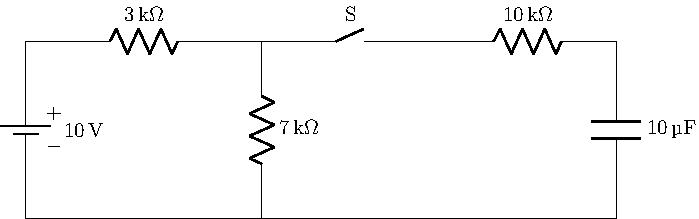
\includegraphics[width = 0.7\columnwidth]{2023/BM/30/figs/c_fig1.pdf}
    \caption{circuit }
    \centering
    \label{fig:bm_30_fig_1}
\end{figure}
\hfill(GATE BM 2023 Question 30)\\
\item 
A finite impulse response (FIR) filter has only two non-zero samples in its impulse response $h[n]$, namely $h[0] = h[1] = 1$. The Discrete Time Fourier Transform (DTFT) of $h[n]$ equals $H(e^{j\omega})$, as a function of the normalized angular frequency $\omega$. For the range $\abs{\omega} \leq \pi$, $\abs{H(e^{j\omega})}$ is equal to
\begin{enumerate}
	\item[(A)] $2\abs{\cos(\omega)}$
	\item[(B)] $2\abs{\sin(\omega)}$
	\item[(C)] $2\abs{\cos(\frac{\omega}{2})}$
	\item[(D)] $2\abs{\sin(\frac{\omega}{2})}$
\end{enumerate}
\hfill(GATE BM 2023 Question 17) \\
\item
For the circuit shown,if $i=\sin 1000t$, the instantaneous value of the Thevenin's voltage(in volts) across the terminals a anb b at time t=5ms is\\[2pt]

\begin{circuitikz}[american voltages,american currents]
    % Draw the circuit components
    \draw (0,0) -- (2,0);
    \draw (2,2) to [resistor,l=$10\Omega$] (2,4);
    \draw (2,4) -- (0,4);
    \draw (2,0) to [capacitor,l=$-j10\Omega$,-,i_=$i_x$] (2,2);
    \draw (2,0) -- (5,0);
    \draw (5,0) to[inductor,l=$j10\Omega$] (5,2);
    \draw (5,2) to [resistor,l=$10\Omega$] (5,4);
  \draw (5,4) to [cV,l^=$4i_x$,invert] (2,4);
  \draw (5,4) -- (6,4);
  \draw (6,4) to[I,l=$\sin 1000t$,invert] (6,0);
  \draw (6,0) -- (5,0);
   \node[circle,fill=black,inner sep=1.5pt,label=above:a] at (0,0) {};
    \node[circle,fill=black,inner sep=1.5pt,label=above:b] at (0,4) {};
    \end{circuitikz}
    \hfill(GATE EE 2023 Question 51) \\
    \pagebreak

    \item In the circuit shown ,$\omega=100\pi\text{rads/s}$, R1=R2=$2.2\Omega$ and L=$7\text{mH}$. the capacitance $\text{C}$ for which $Y_{in}$ is purely real is  $\text{mF}$ \\
	\begin{center}
	\begin{circuitikz} \centering \draw 
		(0,4) to[sinusoidal voltage source, l=$V_{0}$cos($\omega$t)] (0,0)
		(0,4) to[short] (4,4)
		(4,4) to[resistor, l=$R_1$ ] (4,2)
		(4,2) to[inductor, l= $\text{L} $] (4,0) to[short ] (0,0)
		(8,4)  to[short] (4,4)
		(8,4) to[resistor, l= $R_2$] (8,2) to[capacitor,l=$\text{C}$] (8,0) to (4,0);
	\end{circuitikz}
	\end{center}
\hfill(GATE IN 2023 Q46)\\
\solution
\pagebreak

\item The op amps in the circuit are ideal. The input signals are $V_{S1} = 3 + 0.10 \sin(300t), \text{V}$ and $V_{S2} = -2 + 0.11 \sin(300t)\, \text{V}$. The average value of the voltage $V_0$ is \underline{\hspace{1cm}} volts (rounded off to two decimal places).\\
\begin{figure}[ht]
\centering
\resizebox{0.55\columnwidth}{!}{\begin{circuitikz}

% Lines
\draw (-2.5,2.5) -- (0.5,2.5);
\draw (0.5,3) -- (0.5,1);
\draw (0.5,1.5) -- (0,1.5);
\draw (0,1.5) -- (0,0);
\draw (-2.5,-4) -- (0.5,-4);
\draw (0.5,-4.5) -- (0.5,-2.5);
\draw (0.5,-3) -- (0,-3);
\draw (0,-3) -- (0,-1.5);
\draw (0.5,3) -- (2,2);
\draw (0.5,1) -- (2,2);
\draw (2,2) -- (3.5,2);
\draw (3.5,2) -- (5.5,2);
\draw (3.5,2) -- (3.5,1.5);
\draw (0.5,-2.5) -- (2,-3.5);
\draw (0.5,-4.5) -- (2,-3.5);
\draw (2,-3.5) -- (3.5,-3.5);
\draw (3.5,-3.5) -- (3.5,-3);
\draw (3.5,-3.5) -- (5.5,-3.5);
\draw (5.5,-3.5) -- (5.5,-2.25);
\draw (5.5,2) -- (5.5,0.75);
\draw (5.5,-0.75) -- (6.5,-0.75);
\draw (0,0) -- (3.5,0);
\draw (0,-1.5) -- (3.5,-1.5);
\draw (6.5,-1.5) -- (6.5,-2.5);
\draw (6.25,-2.5) -- (6.75,-2.5);
\draw (6.3,-2.55) -- (6.7,-2.55);


% Resistors
\draw (3.5,1.5) to [resistor] (3.5,0);
\draw (3.5,0) to [resistor] (3.5,-1.5);
\draw (3.5,-1.5) to [resistor] (3.5,-3);
\draw (5.5,0.75) to [resistor] (5.5,-0.75);
\draw (5.5,-0.75) to [resistor] (5.5,-2.25);

% Labels
\node at (-3,2.5) {$V_{S1}$};
\node at (-3,-4) {$V_{S2}$};
\node at (0.75,2.5) {+};
\node at (0.75,1.5) {-};
\node at (0.75,-3) {-};
\node at (0.75,-4) {+};
\node at (7,-0.75) {$V_o$};
\node at (4.25,0.75) {R};
\node at (4.25,-0.75) {R};
\node at (4.25,-2.25) {R};
\node at (6.25,0) {R};
\node at (6.25,-1.5) {R};
\node at (6.75,-0.8) {+};
\node at (6.75,-1.5) {-};

% Dot 
\filldraw (6.5,-0.75) circle [radius=0.05];
\fill (6.5,-1.5) circle [radius=0.05]; 

\end{circuitikz}

}
\end{figure}
\hfill{(GATE IN 2023)}
\solution
\pagebreak

\end{enumerate}
